%%%%%%%%%%%%%%%%%%%%%%%%%%%%%%%%%%%%%%%%%%%%%%%%%%%%%%%%%%%%%%%%%%%%%%%%%%%%%%%%%%%%
%% --> ScrewDriver te Blackheadborough:
\newcommand{\AUtoKCM}{627.5084}
\newcommand{\AUtoKJM}{2625.5}
%%%%%%%%%%%%%%%%%%%%%%%%%%%%%%%%%%%%%%%%%%%%%%%%%%%%%%%%%%%%%%%%%%%%%%%%%%%%%%%%%%%%
%% \usepackage{fouriernc}
\newcommand{\Func}[1]{{\ensuremath{\mathcal #1}}}
\newcommand{\AGroup}[1]{{\ensuremath{\mathbb #1}}}
%% ------------------------------------------------| ????
\usepackage{epigraph}
\renewcommand{\epigraphwidth}{7cm}
%\usepackage{pxfonts}
\usepackage{pifont}
\newcommand{\CycleFirst}{\ding{172}}
\newcommand{\CycleSecond}{\ding{173}}
\newcommand{\CycleThird}{\ding{174}}
\newcommand{\CyclePseudoFirst}{\ding{195}}
\newcommand{\CyclePseudoSecond}{\ding{196}}
%%%%%%%%%%%%%%%%%%%%%%%%%%%%%%%%%%%%%%%%%%%%%%%%%%%%%%%%%%%%%%%%%%%%%%%%%%%%%%%%%%%%
%% Пакет, обеспечивающий адекватную расстановку "русских" кавычек
\usepackage[russian]{quotmark}
%% Теперь для точной расстановки русских кавычек по ГОСТ можно использовать 
%% вложенные команды tqt:
%% \tqt{а \tqt{б} в} = ,,а <<б>> в''
%%%%%%%%%%%%%%%%%%%%%%%%%%%%%%%%%%%%%%%%%%%%%%%%%%%%%%%%%%%%%%%%%%%%%%%%%%%%%%%%%%%%
%% Химические пакеты
\usepackage{upgreek}
\usepackage[version=4]{mhchem}
\usepackage{chemfig}
\usepackage{chemmacros}
\usepackage{textgreek}
\chemsetup{modules=all,formula = chemfig,greek=textgreek}
%%%%%%%%%%%%%%%%%%%%%%%%%%%%%%%%%%%%%%%%%%%%%%%%%%%%%%%%%%%%%%%%%%%%%%%%%%%%%%%%%%%% ChemMacros package
%%
\chemsetup[orbital]{
  s/color = blue!75,
  sp3/color = red!75,
  overlay=true,
  opacity=1
}
%%%%%%%%%%%%%%%%%%%%%%%%%%%%%%%%%%%%%%%%%%%%%%%%%%%%%%%%%%%%%%%%%%%%%%%%%%%%%%%%%%%%
\usepackage{chemnum}
\makeatletter
\def\CF@node@content{\expandafter\expandafter\expandafter%
    \printatom\expandafter\expandafter\expandafter%
    {\csname atom@\number\CF@cnt@atomnumber\endcsname}%
    \ensuremath{\CF@node@strut}%
}
\makeatother
\renewcommand*\printatom[1]{\ensuremath{\mathsf{#1}}} % from the ChemFig manual
%% Relied upon \compoundstyle from *chemcompounds*
\usepackage{chemcompounds}
\newcommand{\ConfName}[1]{{\compoundstyle{#1}}}
% Русские...
\newcommand{\BB}[1]{{#1}\ConfName{ВВ}}
\newcommand{\BC}[1]{{#1}\ConfName{ВК}}
\newcommand{\CB}[1]{{#1}\ConfName{КВ}}
\newcommand{\CC}[1]{{#1}\ConfName{КК}}
\newcommand{\TT}[1]{{#1}\ConfName{ТТ}}
%%
%%%%%%%%%%%%%%%%%%%%%%%%%%%%%%%%%%%%%%%%%%%%%%%%%%%%%%%%%%%%%%%%%%%%%%%%%%%%%%%%%%%%
%% chemfig setup
\newcommand{\boldbondwidth}{3.25pt}
\setchemfig{angle increment=15}
\setchemfig{arrow offset=12pt}
\setchemfig{arrow style=thick}
\setchemfig{atom sep=1.75em}
\setchemfig{bond style={line width=1pt}}
\setchemfig{bond offset=2.5pt}
\setchemfig{bond join=true}
\setchemfig{compound sep=4.5em}
\setchemfig{cram width =\boldbondwidth}
\setchemfig{cram dash width=1pt}
\setchemfig{cram dash sep=2pt}
\setchemfig{cycle radius coeff=0.5}
\setchemfig{double bond sep=3pt}
%%
%%%%%%%%%%%%%%%%%%%%%%%%%%%%%%%%%%%%%%%%%%%%%%%%%%%%%%%%%%%%%%%%%%%%%%%%%%%%%%%%%%%%
% подпись на связях в молекуле, нарисованной в пакете *chemfig*
\newcommand\namebond[4][6.5pt]{\chemmove{\path(#2)--(#3)node[midway,sloped,yshift=#1]{#4};}}

\newcommand\arcbetweennodes[3]{%
  \pgfmathanglebetweenpoints{\pgfpointanchor{#1}{center}}{\pgfpointanchor{#2}{center}}%
  \let#3\pgfmathresult}
%%
\newcommand\arclabel[6][stealth-stealth,shorten <=1pt,shorten >=1pt]{%
  \chemmove{%
    \arcbetweennodes{#4}{#3}\anglestart \arcbetweennodes{#4}{#5}\angleend
    \draw[#1]([shift=(\anglestart:#2)]#4)arc(\anglestart:\angleend:#2);
    \pgfmathparse{(\anglestart+\angleend)/2}\let\anglestart\pgfmathresult
    \node[shift=(\anglestart:#2+1pt)#4,anchor=\anglestart+180,rotate=\anglestart+90,inner sep=0pt, outer sep=0pt]at(#4){#6};}
}
%%
\newcommand{\ChemPicture}[1]{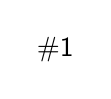
\begin{tikzpicture}\node (ChemFormula) at (0,0){\chemfig{#1}};\end{tikzpicture}}%
%%
%%%%%%%%%%%%%%%%%%%%%%%%%%%%%%%%%%%%%%%%%%%%%%%%%%%%%%%%%%%%%%%%%%%%%%%%%%%%%%%%%%%%%%
%% Немного математических символов
\newcommand{\Energytot}{{\ensuremath E_{tot}}{}}
\newcommand{\Escheme}{\ensuremath{E_{\varpi}}}
\newcommand{\EnergyZPE}{{\ensuremath E_{ZPE}}{}}
\newcommand{\EStrain}{{\ensuremath\Func{E}_\varsigma}{}}
\newcommand{\EConf}{{\ensuremath\Delta\Func{E}_{conf}}{}}
\newcommand{\SymGroup}[2]{\ensuremath{\AGroup{#1}_{#2}}}
%%
%%%%%%%%%%%%%%%%%%%%%%%%%%%%%%%%%%%%%%%%%%%%%%%%%%%%%%%%%%%%%%%%%%%%%%%%%%%%%%%%%%%%%%
\usepackage{pgfplotstable}
\pgfplotsset{compat=1.17}
\pgfplotsset{width=12.5cm}
%\pgfkeys{/pgf/fpu=true}
\pgfplotstableset{%
  1000 sep={},
  empty cells with = {\ensuremath{-}},
  every head row/.style = {before row=\toprule,after row=\midrule},
  every last row/.style = {after row=\bottomrule},
  %every first column/.style={},
  columns/Tau/.style={int detect,column type=r,column type/.add={}{|},column name={$\tau$}},
  columns/Etot/.style={fixed,fixed zerofill,
    column type=r,
    precision=6,column name=$\Energytot{}$},
  columns/Emin/.style={fixed,fixed zerofill,precision=6,
    column name={$E_{min}$},
  },
  columns/Erel/.style={fixed,fixed zerofill,
    column type=r,
    precision=2,%showpos,
    column name={$\Delta\Func{E}$},
    %create on use={create col/expr={2625.5 * {\thisrow{Etot} - \thisrow{Emin}} } },
  }
}
%%%%%%%%%%%%%%%%%%%%%%%%%%%%%%%%%%%%%%%%%%%%%%%%%%%%%%%%%%%%%%%%%%%%%%%%%%%%%%%%%%%%
%% TikZ drawing axes for conformational diagrams:
%%
%%%%%%%%%%%%%%%%%%%%%%%%%%%%%%%%%%%%%%%%%%%%%%%%%%%%%%%%%%%%%%%%%%%%%%%%%%%%%%%%%%%%
%%
\newcommand{\DrawCorrFrame}[2]{%
  \begin{scope}[black]%
    \begin{scope}[thick,solid]
%
      \draw[dashed](0.5,0.) -- (4.5,0.);        % X axis Y=0
      \draw[dotted](0.5,0.38) -- (4.5,0.38);    % k N_A ln 2
      \draw(0.5,#1 - 0.5) -- (0.5,#2 + 0.5);    % Y axis left
      \draw(4.5,#1 - 0.5) -- (4.5,#2 + 0.5);    % Y axis right
      \foreach \y in {#1,...,#2} %
      { %
        \draw(0.45,\y) -- (0.5,\y);%
        \draw(0.45,\y) node [anchor=east] {\small{\y}};
      } %
    \end{scope}%
    \draw(0.5,#2 + 0.5) node[anchor=south] { \(\EConf\) };   % Y axis title
    %\draw(1.0,0.35) [anchor=south,color=black] node{$\confenrg^0$};         % Threshold title
    \foreach \x in {1,...,3}  %
    { %
      \draw[ultra thin,dotted] (\x + 0.5,#1 - 0.25)  -- (\x  + 0.5, #2 + 0.25);%
      %\draw(\x,#1) node[fill=white]{\bfseries{\x}}; % numbers
    } %
  \end{scope}%
}%
%%
%%%%%%%%%%%%%%%%%%%%%%%%%%%%%%%%%%%%%%%%%%%%%%%%%%%%%%%%%%%%%%%%%%%%%%%%%%%%%%%%%%%%%%
%%
\newcommand{\DrawTripleCorrelation}[4]{
% {y(1)}{x}{y(x)}{y(4)}
  \begin{scope}[ultra thick,solid]%
    \draw(0.875, #1) -- (1.125, #1); % #1
    \draw(#2 - 0.125, #3) -- (#2 + 0.125, #3);
    \draw(3.875, #4) -- (4.125, #4); % #4
  \end{scope}%
  % bounding lines
  \begin{scope}%
    \draw(1.125, #1) -- (#2 - 0.125, #3); %
    \draw(#2 + 0.125, #3) -- (3.875, #4); %
  \end{scope}%
}%
%%
%%%%%%%%%%%%%%%%%%%%%%%%%%%%%%%%%%%%%%%%%%%%%%%%%%%%%%%%%%%%%%%%%%%%%%%%%%%%%%%%%%%%%%
%%
\newcommand{\DrawQuadCorrelation}[4]{%
  \DrawTripleCorrelation{#1}{2.0}{#2}{#4}%
  \DrawTripleCorrelation{#1}{3.0}{#3}{#4}%
}
%%
%%%%%%%%%%%%%%%%%%%%%%%%%%%%%%%%%%%%%%%%%%%%%%%%%%%%%%%%%%%%%%%%%%%%%%%%%%%%%%%%%%%%
